% !TEX encoding = UTF-8 Unicode
\documentclass{beamer}

\usepackage{color}
\usepackage{url}
\usepackage[T2A]{fontenc}
\usepackage[utf8]{inputenc}
\usepackage{graphicx}
\usepackage[english,serbian]{babel}
\usepackage{chemfig}
\usepackage[version=3]{mhchem}
\usepackage{multicol}

\mode<presentation>
{
  \usetheme{Warsaw}       % or try default, Darmstadt, Warsaw, ...
  \usecolortheme{default} % or try albatross, beaver, crane, ...
  \usefonttheme{serif}    % or try default, structurebold, ...
  \setbeamertemplate{navigation symbols}{}
  \setbeamertemplate{caption}[numbered]
} 


\definecolor{mygreen}{rgb}{0,0.6,0}
\definecolor{mygray}{rgb}{0.5,0.5,0.5}
\definecolor{mymauve}{rgb}{0.58,0,0.82}

\usepackage{listings}
\lstset{ 
  backgroundcolor=\color{white},
  basicstyle=\scriptsize\ttfamily,
  breakatwhitespace=false,
  breaklines=true,
  captionpos=b,
  commentstyle=\color{mygreen},
  deletekeywords={...},            
  escapeinside={\%*}{*)},          
  extendedchars=true,
  firstnumber=1,              
  frame=single,	                
  keepspaces=true,
  keywordstyle=\color{blue},     
  language=Python,                
  morekeywords={*,...},
  numbers=left, 
  numbersep=4pt,                  
  numberstyle=\tiny\color{mygray}, 
  rulecolor=\color{black},
  showspaces=false,
  showstringspaces=false,
  showtabs=false,
  stepnumber=1, 
  stringstyle=\color{mymauve},
  tabsize=1,
  title=\lstname
}
\usepackage{pgfpages}
\pgfpagesuselayout{resize to}[%
  physical paper width=8in, physical paper height=6in]


% Here's where the presentation starts, with the info for the title slide
\title{F\# na .NET platformi}
\author{T.Todorov T.Garibović D.Nedeljković M.Vićentijević}
\date{\today}

\begin{document}

\begin{frame}
  \titlepage
\end{frame}

% These three lines create an automatically generated table of contents.
\begin{frame}{Pregled}
  \tableofcontents
\end{frame}

\section{Uvod}

\begin{frame}{Uvod}
\begin{itemize}
\item F\# je jezik koji danas ima veoma široku upotrebu
\item Nastao je iz ideje da se strogo tipizirani funkcionalni jezik preusmeri na .NET platformu
\item Autor jezika je Don Sajm (eng.~{\em Don Syme})
\item Pretežno je funkcionalan jezik, ali podržava još dosta programskih paradigmi
\item F\# ima jednostavnu sintaksu, a dovoljno moćnu i za složene matematičke probleme
\item Cilj rada je izdvajanje nekih specifičnih karakteristika
\end{itemize}
\end{frame}

\section{Nastanak i primena jezika F\#}
\subsection*{Poreklo i uticaj drugih jezika}
\begin{frame}{Poreklo i uticaj drugih jezika}

\begin{figure}
\begin{center}
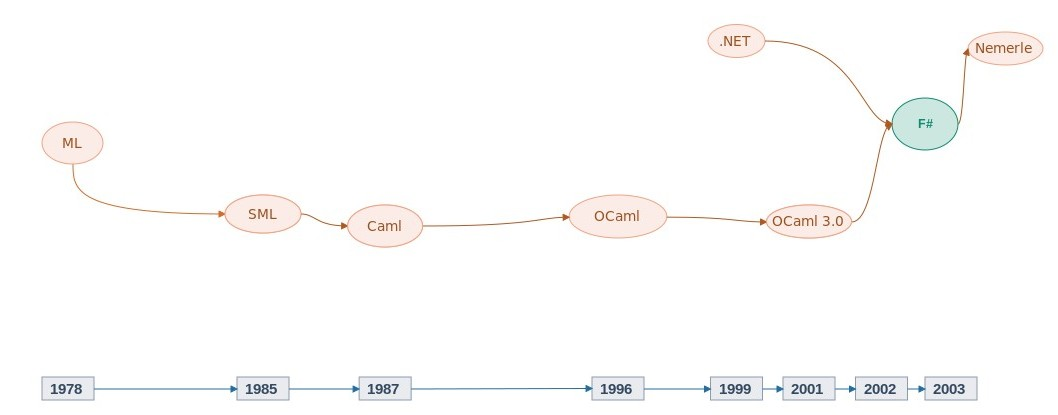
\includegraphics[scale=0.3]{stablo.jpg}
\end{center}
\caption{Razvojno stablo}
\end{figure}

\end{frame}

\subsection*{Primena i mogućnosti}
\begin{frame}{Primena i mogućnosti}

\begin{itemize}
\item Jednostavna sintaksa omogućava laku čitljivost koda
\item Jezik omogućava brzo generisanje prototipova
\item Kôd napisan u F\#-u lako može da se paralelizuje
\item Jezik ima primenu u oblastima: bioinformatika, baze podataka, statistika, finansijsko modelovanje, ...
\item Osim funkcionalnog, jezik F\#, podržava još neke tipove prgramiranja: imperativno, objektono-orjentisano, paralelno, distribuirano, asinhrono, veb programiranje, skript programiranje, ...
\item Koristi se na dosta operativnih sistema: Linux, MAC, Windows, Android, iOS, ...
\end{itemize}

\end{frame}

\section{Osobine i specificnosti jezika}
\begin{frame}{Osobine i specificnosti}
\begin{center}
Osobine: ~~~~~~~~~~~~~~~~~~~~~~~~~~~~~~~~~~ Specificnosti:
\begin{multicols}{2}
\begin{itemize}
  \item Bezbedan
  \item Funkcionalan
  \item Strogo tipiziran
  \item Automatski zakljucuje tipove
  \item Kompatibilan
  \item Povratna vrednost if/else
  \item Opciono - return
  \item Kljucne reci let i mutable
  \item Pattern matching
  \item Novi tip option type
\end{itemize}
\end{multicols}
\end{center}
\end{frame}

\section{Funcionalna paradigma - Pattern matching}  
\begin{frame}[fragile]
\frametitle{Funcionalna paradigma - Pattern matching}

\begin{itemize}
  \item Glavna paradigma programskog jezika F\#
\end{itemize}

\begin{block}{Pattern matching}
Pattern matching je mehanizam koji koristi dekompoziciju i kontrolu toka podataka za poklapanje obrazaca koriscenjem navedene konstrukcije:
\textbf{ match ... with ...}
\begin{lstlisting}
let urlFilter url agent =
 match (url,agent) with
 | "http://www.control.org", 99 -> true
 | "http://www.kaos.org" , _ -> false
 | _, 86 -> true
 | _ -> false
\end{lstlisting} 
\end{block}

\end{frame}

\section{Asinhrono i paralelno programiranje}
\begin{frame}[fragile]
\frametitle{Asinhrono i paralelno programiranje}



\end{frame}

\section{Radni okvir - .NET framework}
\begin{frame}[fragile]
\frametitle{Radni okvir - .NET framework}
Temelj .NET platforme je zajednicka jezicka infrastruktura CLI({\em(Common Language Infrastructure)}.Kodovi se prevode na MSIL({\em Microsoft Intermediate Language}) alemblerski jezik.\\
Implementacija MSIL-a na CLI kompajleru je brza i ima sledece prednosti u odnosu na masinski:
\begin{itemize}
	\item kompatibilnost medju jezicima
	\item mogucnost rada na vise platformi
	\item masinska nezavisnost
\end{itemize}
Mogucnost automatskog prikupljanja smeca je jos jedna prednost.
Jos neki okviri: veb radni okviri({\em Suave, Fable, ASP.NET Core}...) i radni okviri za testiranje veba ({\em Web Testing, Frameworks, Unit Testing Libraries}...)
\end{frame}

\section{Instalacija i pokretanje}
\begin{frame}[fragile]
\frametitle{Instalacija i pokretanje}

\begin{itemize}
\item Alati koji na Windows-u podrzavaju F\# se instaliraju u nekoliko koraka:
	\begin{itemize}
	\item Visual Studio Code
	\item Visual studio
	\item JetBrains Rider
	\end{itemize}
\item Na Linux-u se instalacija vrsi na isti nacin za sledece verzije:
	\begin{itemize}
	\item Ubuntu
	\item Mint
	\item Debian
	\end{itemize}
	\item \begin{lstlisting}
fsharpc primer.fs
\end{lstlisting}
\end{itemize}
\end{frame}

\section{Fizz Buzz}
\begin{frame}[fragile]
\frametitle{Fizz Buzz}

\begin{lstlisting}
let (|Fizz|Buzz|FizzBuzz|Other|) n =
    match (n % 3, n % 5) with
    | 0, 0 -> FizzBuzz
    | 0, _ -> Fizz
    | _, 0 -> Buzz
    | _ -> Other n

let fizzBuzz =
    function
    | Fizz -> "Fizz"
    | Buzz -> "Buzz"
    | FizzBuzz -> "FizzBuzz"
    | Other n -> n.ToString()

seq { 1..100 } |> Seq.map fizzBuzz|> Seq.iter (printfn "%s")
\end{lstlisting}

\end{frame}

\section{Jedinica mere}
\begin{frame}[fragile]
\frametitle{Jedinica mere}

\begin{itemize}
  \item Pad orbitera poslatog na Mars 1999.
  \begin{itemize}
  	\item Uzrokovan cinjenicom da je deo softvera koristio numericke, a deo softvera engleske jedinice
  \end{itemize}
  \item Prevencija gresaka na osnovu konteksta primene
  \begin{itemize}
  	\item Numerickim tipovima se pridruzuju metapodaci
  	\item Kompajler na osnovu metapodataka proverava ispravnost
  \end{itemize}
  \item Jedinstveno svojstvo jezika F\#
  \item Primer definisanja jedinice mere  
\begin{lstlisting}
  [<Measure>] type cm
  [<Measure>] type inch  
\end{lstlisting}
\end{itemize}
\end{frame}

\begin{frame}[fragile]
\frametitle{Jedinica mere}

\begin{lstlisting}
[<Measure>] type rsd
[<Measure>] type eur
[<Measure>] type hour
[<Measure>] type week
[<Measure>] type year

let hoursBilledPerWeek = 40.0<hour/week>
let weeksWorkedPerYear = 35.0<week/year>
let rsdPerHour = 1000.0<rsd/hour>
let exchangeRate = 0.008547<eur/rsd>

let eurPerYear = rsdPerHour * hoursBilledPerWeek * weeksWorkedPerYear * exchangeRate
let bonus = 500.0<eur/year>

printfn "%f" (eurPerYear + bonus)
\end{lstlisting}
\cite{progFs}
\end{frame}

\section{Literatura}

\begin{frame}{Literatura}

\bibliography{primer1.bib}

\end{frame}

\end{document}